\textbf{Name: Patrick Harvey} \\

\medskip

\textbf{Conspirators: Christopher O'Neil} 

\medskip
\medskip

\hrule

\medskip


\assignmentsonly{\pleasesubmitprojectdraft}

\begin{itemize}
\item 
  Please use Overleaf for writing up your project.
\item
  Build your paper using:
  \url{https://github.com/petersheridandodds/universal-paper-template}
\item
  Please use Github and Gitlab to share the code and data things you make.
\item
  For this first assignment, just getting the paper template up is enough.
\end{itemize}

\solutionstart

The template for this paper can be found at: \url{https://github.com/P-Harvey/papers/tree/main/2023-05supply-optimization}


\solutionend

\begin{enumerate}
  
\item
  
  Come up with some rich, text-based stories for analysis.

  For example: One (longish) book, or a book series, or a TV series.

  Data would be the original text (books), subtitles, screenplay, or scripts (TV series).

  \begin{itemize}
  \item 
    You must be able to obtain the full text.
  \item 
    You will want something with at least around $10^{5}$ words.
    More than $10^{6}$ would be great.
  \item 
    Transcripts of shows may be good for extracting
    temporal character interaction networks.
  \end{itemize}

  Please talk about possibilities with others in the class.
  
  For this assignment, simply list at least one possibility, noting the approximate text size
  in number of words.

  \solutionstart
  
  For this problem I have selected the book "Blood  Meridian" by Cormac McCarthy\cite{mccarthy_1985}, which has greater than $10^4$ unique words after pre-processing the text for punctuation and white-space.
  
  The initial examination of this text can be found at  \url{https://github.com/P  Harvey/csys303_assignments/blob/642aae80fb5d5627a5acd  203fe1a0374310c8fc/plharvey_15/plharvey_15.ipynb}.
  
  \solutionend

\item   
  Tokunaga's law is statistical but we can consider
  a rigid version.  Take $T_1 = 2$ and $R_T = 2$ and
  draw an example network of order $\Omega=4$ with these parameters.

  Please take some effort to make your network look somewhat like a river network.

   \solutionstart
   \begin{figure}[!htpb]
       \centering
       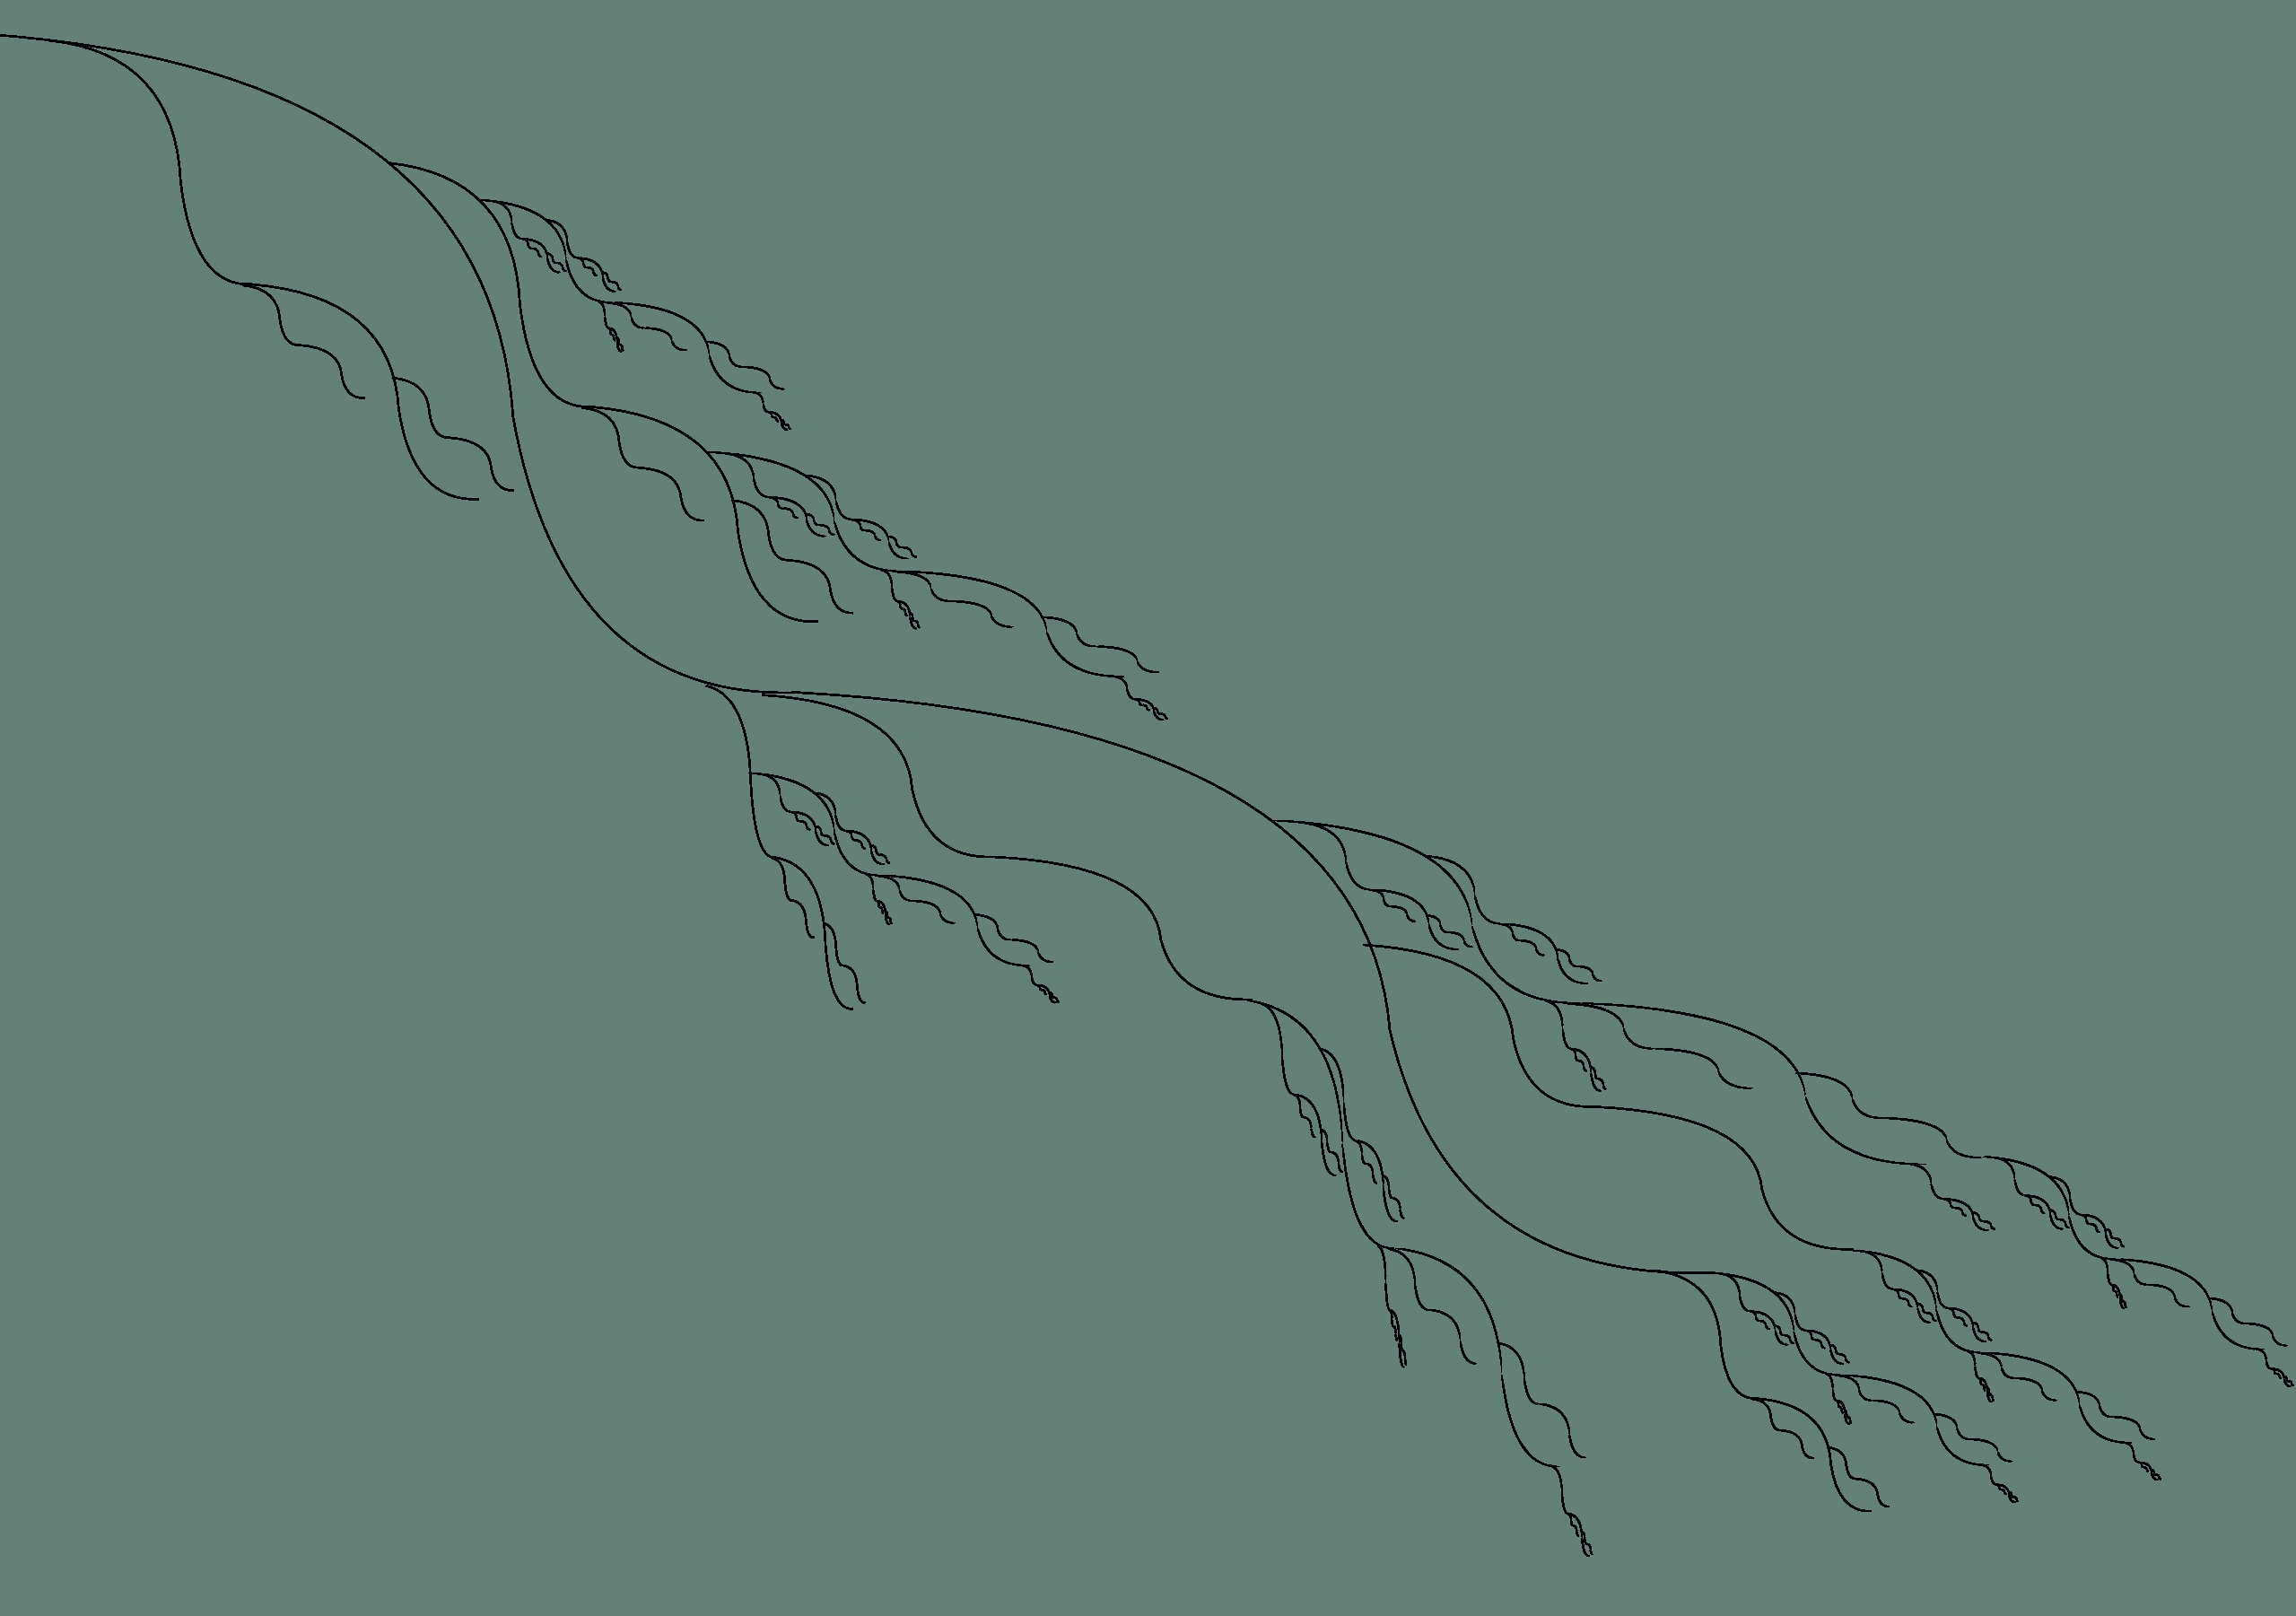
\includegraphics[width=\textwidth]{15_2.jpeg}
       \caption{Branching network with $T_1 = 2$ and $R_T = 2$ of order $\Omega=4$.}
       \label{fig:15_2}
   \end{figure}
   \solutionend

  
\item Show $R_\okell = R_\msl$.  In other words show that Horton's law of
  stream segments matches that of main stream lengths, and do
  this by showing they imply each other.

  
   \solutionstart

   Let $R_s = \frac{\bar{s}_{\omega+1}}{\bar{s}_{\omega}}$

   then:
   \begin{align}
       \bar{s}_{\omega+1} &= \bar{s}_{\omega}R_s\\
       &= \bar{s}_{\omega-1}(R_s)^2\\
       &= \bar{s}_{\omega-2}(R_s)^3\\
       &\cdots\\
       &= \bar{s}_{1}(R_s)^{\omega}\\
   \end{align}
   
   In other words: if we take this as a bifurcation ratio ($R_b = \frac{1}{\alpha}$ also expressed as $R_b = \frac{n_i}{n_i + 1}$), and raise it to the $N-1^{\text{th}}$ power, then we have a function that lineally maps $x$ to $n$ ($R_{b}^{N-1} \therefore n(x)=ax^b$).

   If we take the average length of order $\omega$:

   \begin{align}
       \bar{\ell}_{\omega} &= \sum^{\omega}_{i=1}{\bar{s}_i}\\
       &= \bar{s}_1 + \cdots + \bar{s}_{\omega}\\
       &= \sum_{i=1}^{\omega}{R^{i-1}_{s}\bar{s}_1}\\
       \therefore \bar{\ell}_{\omega} &= \bar{s}_1\frac{1-R_{s}^{\omega}}{1-R_s} \text{for} R_s \neq 1\\
   \end{align}

   If we assume that $R_\ell = \frac{\bar{\ell}_{\omega+1}}{\bar{\ell}_\omega}$, then we have $\bar{s}_\omega = \bar{\ell}_\omega - \bar{\ell}_{\omega-1}$

   \begin{align}
       \frac{\bar{s}_{\omega+1}}
       {\bar{s}_{\omega}}
       &= \frac{\bar{\ell}_{\omega+1} - \bar{\ell}_{\omega}}
       {\bar{\ell}_\omega - \bar{\ell}_{\omega-1}}\\
       &= \frac{\bar{\ell}_1 R_{\ell}^{\omega} - \bar{\ell}_1 R_{\ell}^{\omega-1}}
       {\bar{\ell}_1 R_{\ell}^{\omega-1} - \bar{\ell}_1 R_{\ell}^{\omega-2}}\\
       &= \frac{R_{\ell}^{\omega} - R_{\ell}^{\omega-1}}
       {R_{\ell}^{\omega-1} - R_{\ell}^{\omega-2}}\\
       &= \frac{R_{\ell}^{\omega-1}(R_\ell - 1)}
       {R_{\ell}^{\omega-2}(R_\ell - 1)}\\
       &= R_\ell\\
       \therefore R_s & = R_\ell\\
   \end{align}

   \solutionend


\end{enumerate}